% UNIT : Overview of ML approaches to Cog Neuro 
\chapter{Overview of ML approaches to modeling cognitive neuroscience data}
\label{chap:overview}

In this Chapter we have two papers on the topic of \textbf{cognitive neuroscience models}.

\section[Analyzing biological and artificial neural networks]{\textit{Analyzing biological and artificial neural networks: challenges with opportunities for synergy?}\\ \mandatory{BARRETT201955}}

Deep neural networks brought a revolution in the area of ML, with millions of parameters, no engineered features, and very high performance. We can see an \textbf{analogy with neuroscience}, as both fields need to:
\begin{itemize}
    \item understand how neural networks, consisting of large numbers of interconnected elements, transform representations of stimuli across multiple processing stages to implement a wide range of complex computations and behaviours;
    \item describe and analyze very high dimensional data.
\end{itemize}

The analogies appear in four areas: Receptive fields, Ablation, Dimensionality reduction, and Representational geometries.

\subsection{Receptive fields}
Neurons in the human visual cortex are \textbf{specialized to process stimuli in specific spatial areas} (see \notedv Retinotopy map) \textbf{or certain types of features}.
The neurons in the \textbf{initial processing} regions of the visual cortex have \textbf{small receptive fields}; sensitive to stimuli in small areas of visual space.
As information is transmitted to \textbf{higher level} areas of visual processing, \textbf{receptive fields become larger}, enabling sensitivity to larger areas of space. These regions also encode more complex features, and there is evidence of ``abstract" coding with invariance to small transformations. There are ``\textbf{concept cells}” \textbf{sensitive to identity} of objects but \textbf{not to appearance}. For example, simple ``repetition priming \notet" effect repeated exactly with same face but different orientation.
\osst{Repetition priming refers to the change in responding to a word or an object as a result of a previous encounter with that same item, either in the same task or in a different task.}

(Some) AI researchers also think that \textbf{DNN neurons may code for specific information}, which can be studied via receptive field analysis.

Some experiments investigate which types of images maximally activate a neuron. Other studies examine how receptive fields change in deeper layers (as we go deeper in the network, each element in the feature map is occupying more space in the visual field, through pooling, but \textit{in what way are larger receptive fields more complex?}).
\begin{figure}
    \centering
    \captionsetup{width=.8\linewidth}
    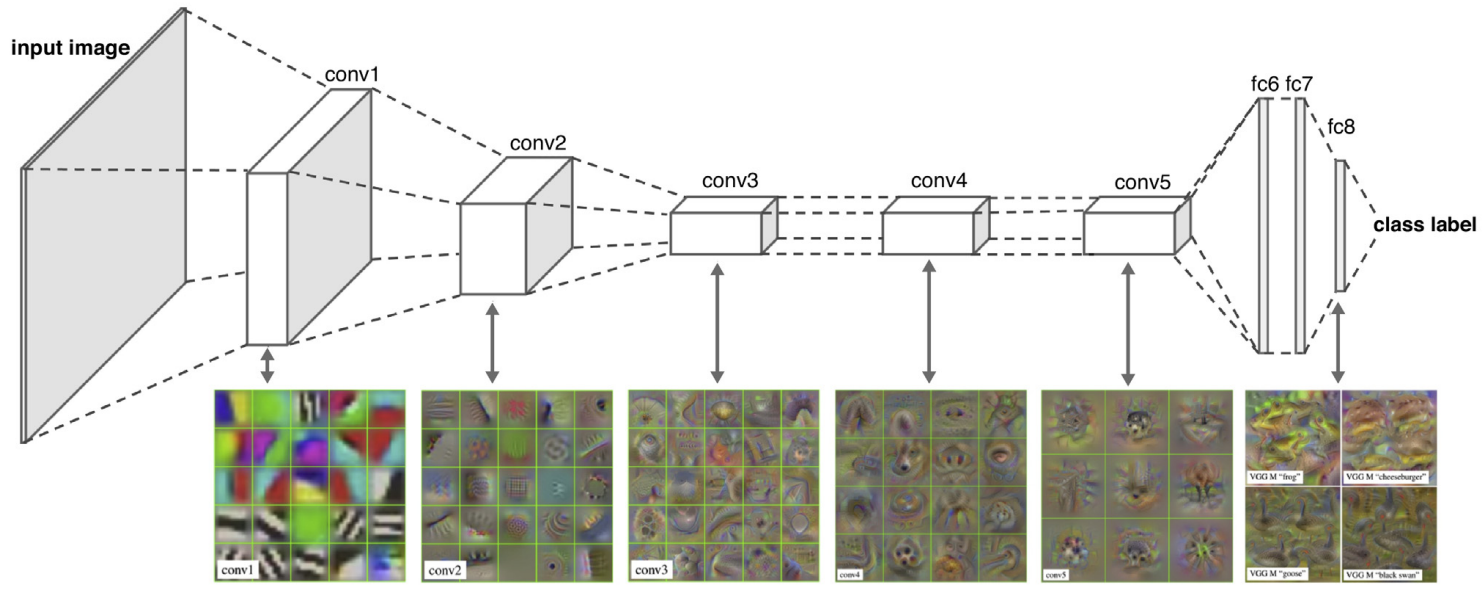
\includegraphics[width=1\linewidth]{images/dnn_receptive_fields.png}
    \caption{Top: how an input image is progressively processed by a CNN. Bottom: receptive fields for each layer are calculated using activation maximization (i.e. take an already trained CNN and create stimuli that produce the maximal activation in a given feature mapping in the network). For each layer, a single square corresponds to a feature map. We can notice \texttt{conv1} (the first layer) encodes large scale information; some shapes (e.g. circles) start appearing as early as \texttt{conv2}.}
\end{figure}

\boxl{Retinotopy map}{
The \textbf{oxcipital cortex} (\textbf{visual cortex}) is devoted to image processing. They found out that the coding in the brain is along two dimensions: \textbf{eccentricity} and \textbf{radial degree}.
It is possible to get a map of such coding by applying fMRI to a relatively simple experiment:

\begin{center}
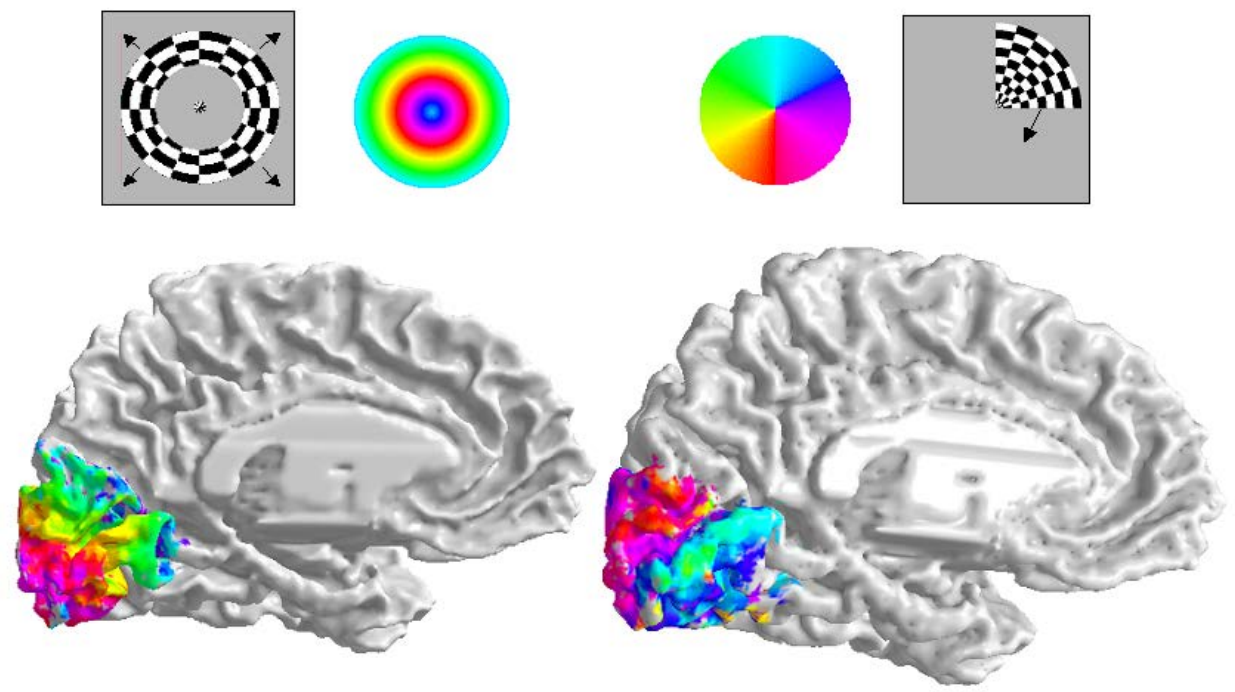
\includegraphics[width=0.7\textwidth]{images/retinotopy.png}
\end{center}
Focus first on the experiment on the left. The person is looking at the center of the shape. While looking, the shape changes according to a defined temporal pattern (shrinking and expanding with a certain period). If there are neurons caring for a certain distance from the center, then they should fire at determinate time points. This is indeed the case, and we can track which neurons code for a certain eccentricity (we use colors to represent eccentricity).

The experiment on the right is quite similar: while the person is looking at the center, the shape rotates around it.

Different people have almost all the same coding, and it is interesting to note how there are no ``jumps" in the coding.\\

A similar thing can be done with the \textbf{primary auditory cortex}, in the \textbf{temporal lobe}, to get a \textbf{tonotopy map}.
}

\subsection{Ablation}
Brain lesions (ablations) offer much information about potential function of brain areas. By mapping lesions to symptoms, we can understand which brain areas are important for given tasks.

\begin{wrapfigure}[13]{r}{0pt}
  \centering
  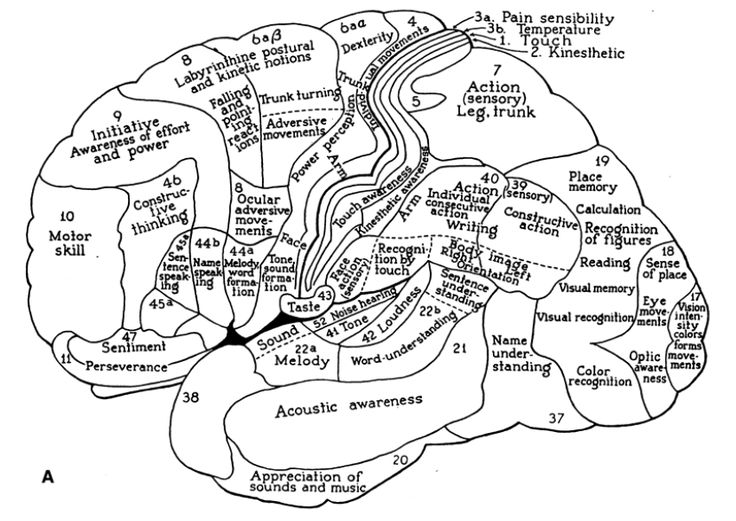
\includegraphics[width=0.4\textwidth]{images/kleist.png}
  \caption*{Kleist's functional brain map. This map is old and partially incorrect, but still interesting.}
\end{wrapfigure}

Pruning and ablation causes performance deficits. However, thanks to neuroplasticity, the human brain can achieve again the same performance.\\

Speaking of artificial neural networks, the debate in the last years has seen three thesis on how DNNs encode information:
\begin{itemize}
    \item distributed information (meaning we can remove some parts without hardly impacting a single task),
    \item local encoding (meaning some neurons are super specialized and don't share encoding information),
    \item Modularity theory: not each single neuron is necessary, but some modules (groups of neurons) are necessary for specific tasks.
\end{itemize}

We ask ourselves, how do artificial neural networks change after ablation?
The ablation (lesioning) analysis is applicable to DNNs. We can \textit{silence} neurons and observe how this impacts the network output. Silencing of neurons is done via \textbf{structural pruning} (entirely removing a neuron with all its outgoing weights).
Networks trained for generalization (out of sample prediction) are more robust to ablation than those trained on memorizing labels. 
Pruning and fine-tuning are active areas of research.

\subsection{Dimensionality reduction}
The brain codes information in a distributed manner, necessitating 
multivariate analysis:
\begin{itemize}
    \item Multiple units encode information in the brain, leading to \textbf{redundancy} where two neurons may fire almost identically; or
    \item Information is coded in a \textbf{distributed} manner among multiple units (e.g. coding for 4 classes among 2 neurons, each coding $\{0,1\}$); or 
    \item \textbf{Correlation} among units could indicate that the \textbf{activity can be described in a lower dimensional space}.
\end{itemize}

It has been shown that, in DNNs, an object-by-feature matrix from fully connected layer can be \textbf{compressed by more than 80\%} (e.g. from 4096 dimensions to 512) while maintaining almost all variance. This means few dimensions are enough to explain differences between images. 

\subsection{Representational geometries}
To \textbf{understand representations}, we study how they are represented in different layers, how they change over time, and how are different embedding spaces related to each other.

\paragraph{Matrix factorization measures:} they are a good starting point to compare matrices and understand if there is some sort of covariance between the two. We compare representations across networks by comparing \textbf{object-by-feature matrices}. \textit{Canonical Correlation Analysis} and \textit{PLScorrelation} are two different factorization measures, they identify lower-level factors that capture and maximize the correlations/covariance between the datasets (note: these methods can be seen as ``supervised" as they re-weight columns in both tables to maximize similarity).

\paragraph{Representational Similarity Analysis:} it involves \textbf{comparing two similarity matrices}, often constructed from object-by-feature matrices. This yields an object-by-object similarity matrix.
Representational Similarity Analysis does not factorize matrices. The principle is: describe how the objects cluster together (in the representational space) according to the matrix. To code for distances between objects, we need a distance matrix; and to get this a distance function is needed (e.g. Euclidean, Mahalanobis, etc.), indeed each row in the object-by-feature matrix is a vector. So we can \textbf{turn the object-by-feature matrix into an object-by-object distance matrix} (pairwise distance between objects).
For human data (how human represent things), we usually don't get an object-by-feature matrices (we are directly provided an object-by-object matrix), so with RSA we can study the \textbf{relationship between human representation and machine representation}.

\paragraph{Linear regression:} The machine representation in the neural network (\textit{DNN embeddings}) can be used to predict brain activity (\textit{neurobiological activation vectors}) using linear regression.

\section[Spatial methods, Logical methods and Artificial neural networks]{\textit{What does the mind learn? A comparison of human and machine learning representations}\\ \mandatory{SPICER201997}}

This paper reviews the modern machine learning techniques and their use in models of human mental representations, detailing three notable branches: spatial methods, logical methods and artificial neural networks.
\begin{figure}[ht]
    \centering
    \captionsetup{width=.8\linewidth}
    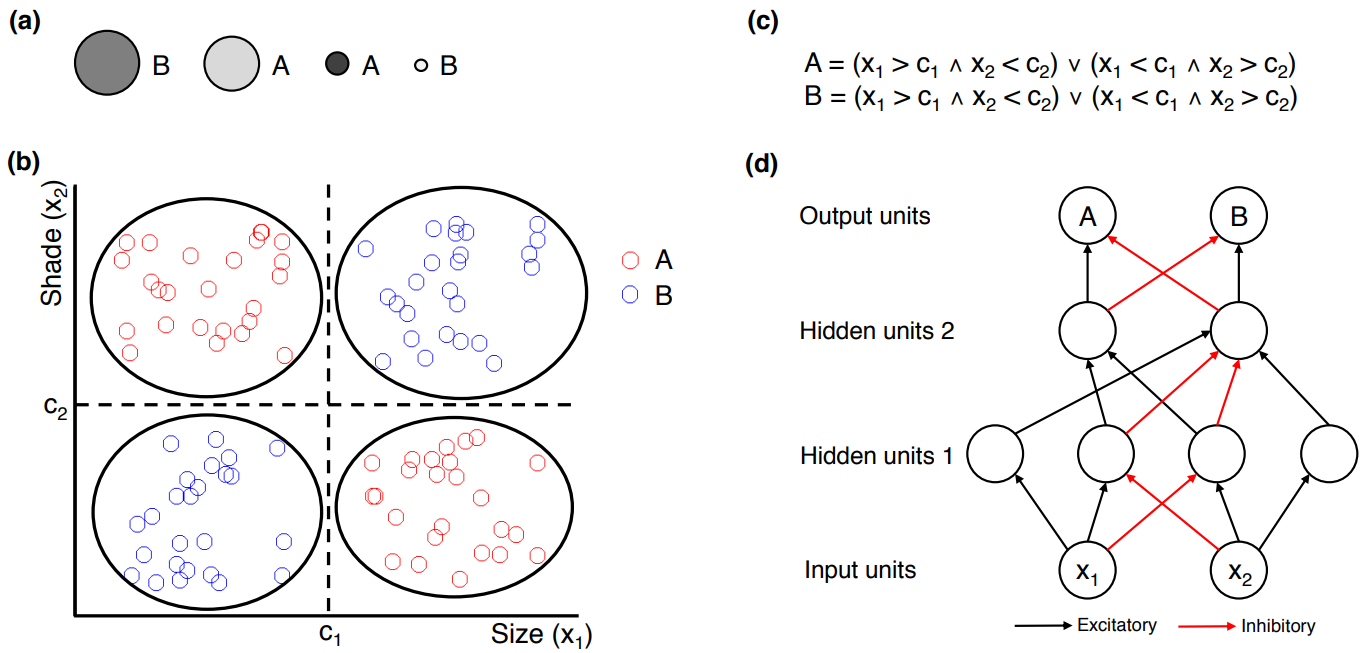
\includegraphics[width=0.75\linewidth]{images/xor.png}
    \caption{Illustration of the XOR classification task using size and shade: examples of stimuli in \textbf{(a)}. This problem can be solved by a spatial clustering method \textbf{(b)}, a logical Boolean method \textbf{(c)}, and an artificial neural network \textbf{(d)}.}
\end{figure}

\subsection{Spatial methods}
Spatial methods involve placing items in a \textbf{multidimensional space} and using their location to draw conclusions about \textbf{categorization}.
Classification based on spatial methods can be determined by an item's location relative to a hyperplane or its similarity to different prototypes (means) or exemplars (centroids):
\begin{itemize}
    \item \textbf{Prototype approaches} assume that learning is based on similarity to the center of a category (mean), which is stored after training (i.e. all examples are forgotten, the prototype only is stored).
    \item \textbf{Exemplar approaches} calculate similarity as a ratio between the similarity of an item to all items within a class (i...n) and the similarity of that item to all other items. This provides a fit per class and requires storing item-level information (i.e. all examples are kept).
    \item \textbf{Clustering} organizes items into groups (cohorts), with quality often quantified by the distance between items within and between clusters. Clustering can be either hard (each item belongs to only one cluster) or soft (items can have multiple memberships, potentially fuzzy).
\end{itemize}

\boxc{Example of spatial method: Generalized Context Model (GCM)}{
According to the GCM, the probability that stimulus $i$ is classified into category $C_J$ is found by summing the similarity of $i$ to all training exemplars of $C_J$ and then dividing by the summed similarity of $i$ to all training exemplars of all categories:
\[
P(C_J|i )= \frac{ \left( \sum_{j \in J} s_{ij} \right)^\gamma }
{\sum_K \left( \sum_{k \in K} s_{ik} \right)^\gamma} 
\]
}

\subsection{Logical methods and Artificial neural networks (ANNs)}
\paragraph{Logical methods:} concepts are based on a definition that is applied to the features of the object. One viable solution is searching for rules that maximize discrimination between stimuli; the rules can be probabilistic (i.e., the rules, if not given, can be automatically computed/learned).

\paragraph{ANNs:} do not make assumptions about the representations involved, but offer an implementation method.

\subsection{Thoughts}
Asking which model is the most accurate might be misleading: the answer depends on what area of science you work in. Therefore it is better to focus on whether a model offers ``useful explorations of the ways in which human learning operates”.
The value depends not just on match to human behavior, but whether there is a need to understand the underlying representations. We have to consider \textbf{not just accuracy}, but \textbf{also confusion}.
Today, very large emphasis is put on \textbf{explainability}: we want to explain the model behaviors (for naturally explainable models). And if it is not naturally explainable, we need to address this issue.
